\documentclass[12pt,openany]{book}


\usepackage{amsmath,amsthm,amsfonts,amscd} % Packages for mathematics

% Colors
\usepackage[dvipsnames]{xcolor}
\definecolor{titleblue}{RGB}{0,53,128}
\definecolor{chaptergray}{RGB}{140,140,140}
\definecolor{sectiongray}{RGB}{180,180,180}

% Fonts
\usepackage[T1]{fontenc}
\usepackage[utf8]{inputenc}
\usepackage{newpxtext,newpxmath}
\usepackage{sectsty}
\allsectionsfont{\sffamily\color{titleblue}\mdseries}

% Page layout
\usepackage{geometry}
\geometry{a4paper,left=1.5in,right=1in,top=1in,bottom=1in,heightrounded}
\usepackage{fancyhdr}
\fancyhf{}
\fancyhead[LE,RO]{\thepage}
\fancyhead[LO]{\nouppercase{\rightmark}}
\fancyhead[RE]{\nouppercase{\leftmark}}
\renewcommand{\headrulewidth}{0.5pt}
\renewcommand{\footrulewidth}{0pt}

% Chapter formatting
\usepackage{titlesec}
\titleformat{\chapter}[display]
{\normalfont\sffamily\Huge\bfseries\color{titleblue}}{\chaptertitlename\ \thechapter}{20pt}{\Huge}
\titleformat{\section}
{\normalfont\sffamily\Large\bfseries\color{chaptergray}}{\thesection}{1em}{}
\titleformat{\subsection}
{\normalfont\sffamily\large\bfseries\color{sectiongray}}{\thesubsection}{1em}{}

% Table of contents formatting
\usepackage{tocloft}
\renewcommand{\cftchapfont}{\sffamily\color{titleblue}\bfseries}
\renewcommand{\cftsecfont}{\sffamily\color{chaptergray}}
\renewcommand{\cftsubsecfont}{\sffamily\color{sectiongray}}
\renewcommand{\cftchapleader}{\cftdotfill{\cftdotsep}}

% Hyperlinks
\usepackage{hyperref}
\hypersetup{
	colorlinks=true,
	linkcolor=titleblue,
	filecolor=black,      
	urlcolor=titleblue,
}

%---------------------------My Preamble
\usepackage{graphicx}
\usepackage{tikz-cd}
\usetikzlibrary{decorations}\usepackage{enumerate}

\usepackage{xcolor}
\usepackage{soul}
\newcommand{\mathcolorbox}[2]{\colorbox{#1}{$\displaystyle #2$}}


%Tcolorbox
\usepackage[most]{tcolorbox}
%\tcbset{colback=white,colframe=black,fonttitle=\bfseries,arc=4mm,boxrule=1pt,shadow={2mm}{-1mm}{0mm}{black!50}}
\tcbset{enhanced, colback=white,colframe=black,fonttitle=\bfseries,arc=4mm,boxrule=1pt,shadow={2mm}{-1mm}{0mm}{black!50}}
%drop shadow

%White box with black text and shadow
%\begin{tcolorbox}[colback=white,colframe=black,fonttitle=\bfseries,title=Black Shadow Box,arc=4mm,boxrule=1pt,shadow={2mm}{-1mm}{0mm}{black!50}]
%	This is a white box with black text and a subtle shadow. The shadow adds some depth and dimension to the box without overpowering the design.
%\end{tcolorbox}

%Theorem
%\usepackage{amsthm}
\newtheorem{axiom}{Axiom}[section]
\newtheorem{theorem}{Theorem}
\newtheorem{proposition}[theorem]{Proposition}
\newtheorem{corollary}{Corollary}[theorem]
\newtheorem{lemma}[theorem]{Lemma}

\newtheorem{definition}{Definition}
\newtheorem{remark}{Remark}
\newtheorem{exercise}{Exercise}[section]

%New Command
\newcommand{\set}[1]{\left\{#1\right\}}
\newcommand{\N}{\mathbb{N}}
\newcommand{\Z}{\mathbb{Z}}
\newcommand{\Q}{\mathbb{Q}}
\newcommand{\R}{\mathbb{R}}
\newcommand{\C}{\mathbb{C}}
\newcommand{\F}{\mathbb{F}}
\newcommand{\nbhd}{\mathcal{N}}

\newcommand{\of}[1]{\left( #1 \right)} 
\newcommand{\abs}[1]{\left\lvert #1 \right\rvert}
\newcommand{\norm}[1]{\left\| #1 \right\|}

\newcommand{\sol}{\textcolor{magenta}{\bf Sol}}

% Begin document
\begin{document}
	
	% Title page
	\begin{titlepage}
		\begin{center}
			{\Huge\textsf{\textbf{Complex Analysis}}\par}
			\vspace{0.5in}
			{\Large Ji Yong-Hyeon\par}
			\vspace{1in}
			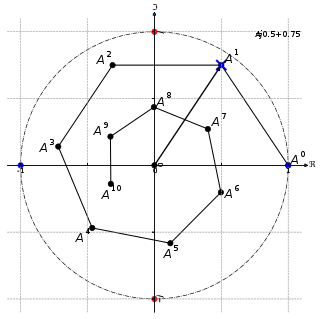
\includegraphics[width=3in]{Exponentials_of_complex_number_within_unit_circle-2.png}\par
			\vspace{1in}
			{\large Ji Yong-Hyeon\par}
			{\large \today\par}
		\end{center}
	\end{titlepage}
	
	% Table of contents
	\tableofcontents
	
	% Chapters
	\mainmatter
	
	\chapter*{Continuity and Derivatives}
	
	\section*{Continuity}
	\begin{tcolorbox}[title=Continuity]
	\begin{definition}
		Let $\varnothing\neq S(\subseteq\R)$. Let $f:S\to\R$ be a real function, and let $\alpha\in S$. We say that \textbf{$f$ is continuous at $\alpha$} if \[
		\forall\varepsilon>0:\exists\delta>0\quad\text{s.t.}\quad\abs{x-\alpha}<\delta\implies\abs{f(x)-f(\alpha)}<\varepsilon.\footnote{$\iff \forall\varepsilon>0:\exists\delta>0\ \text{s.t.}\ f\left(\nbhd_\delta(\alpha)\right)\subseteq\nbhd_\varepsilon\left(f(\alpha)\right)$.}
		\] In other words, \[
		\lim\limits_{x\to\alpha}f(x)=f(\alpha).
		\] If $f$ is continuous on every point of $S$, then $f$ is called a \textbf{continuous function on $S$}.
	\end{definition}
	\end{tcolorbox}
	\begin{remark}
	$f$ is discontinuous at $\alpha$ if and only if \begin{align*}
	&\exists\varepsilon>0\quad\text{s.t.}\quad\forall\delta>0:\abs{x-\alpha}<\delta\ \text{but}\ \abs{f(x)-f(\alpha)}\geq\varepsilon\\
	\iff &\exists\varepsilon>0\quad\text{s.t.}\quad\forall\delta>0:\nbhd_\varepsilon\left(f(\alpha)\right)\subset f\left(\nbhd_\delta(\alpha)\right).
	\end{align*}
	\end{remark}


	\begin{tcolorbox}[colback=white!10!white,colframe=blue!50!black,title=Continuity]
		A function $f:S(\neq\varnothing)\to\R$ is continuous at $\alpha\in S$ iff \[
		\varepsilon\in\R^+\implies\exists\delta\in\R^+:[f\left[\nbhd_\delta\of{\alpha}\right]\subseteq\nbhd_\varepsilon\of{f\of{\alpha}}].
		\]
	\end{tcolorbox}

	\begin{tcolorbox}[colback=red!5!white,colframe=red!75!black,title=Warning]
		This is a warning box. It can be used to alert readers to potential dangers or problems.
	\end{tcolorbox}

	\begin{tcolorbox}[colback=white!10!white,colframe=black!50!white,title=Tabular Box,fonttitle=\bfseries\large,sharp corners]
		\begin{tabular}{|c|c|c|}
			\hline
			1 & 2 & 3 \\
			\hline
			4 & 5 & 6 \\
			\hline
			7 & 8 & 9 \\
			\hline
		\end{tabular}
	\end{tcolorbox}

	
	The continuity of a function is a fundamental concept that describes the behavior of a function near its domain. A function is said to be continuous at a point $x_0$ in its domain if the limit of the function as $x$ approaches $x_0$ exists and is equal to the function value at $x_0$.
	
	The formal definition of continuity of a function $f(x)$ at a point $x_0$ is:
	
	\begin{align*}
		\lim_{x \to x_0}f(x) &= f(x_0)\
	\end{align*}
	
	That is, the limit of $f(x)$ as $x$ approaches $x_0$ exists and is equal to $f(x_0)$.
	
	If a function is continuous at every point in its domain, then it is said to be a continuous function. There are different types of continuity, such as pointwise continuity, uniform continuity, and local continuity.
	
	Pointwise continuity means that the function is continuous at each point in its domain. Uniform continuity means that the function has a continuous behavior over the entire domain, without any abrupt changes or jumps. Local continuity means that the function is continuous in a small neighborhood around each point in its domain.
	
	The concept of continuity is important in the analysis of functions, and it plays a crucial role in the study of limits, derivatives, and integrals. The continuity of a function also helps us understand its behavior, including the existence of critical points, extreme values, and asymptotic behavior.
	
	In summary, the continuity of a function is a crucial concept in mathematical analysis, and it is essential for understanding the behavior of functions near their domain.
	
	\newpage
	\section{Derivatives}
	\begin{tcolorbox}[title=Differentaible Mapping]
		\begin{definition}
			Let $f:I\to\R$ on an interval $I$ and $\alpha\in I$. A real function $f$ \textbf{is differentiable at the point $\alpha$} if and only if either the limit \[
			f'(\alpha):=\frac{df}{dx}\bigg|_{x=\alpha}:=\mathcolorbox{-blue}{\lim_{x\to\alpha}\frac{f(x)-f(\alpha)}{x-\alpha}}\quad\text{or}\quad \mathcolorbox{-blue}{\lim_{h\to0}\frac{f(\alpha+h)-f(h)}{h}}
			\] exists. Here, $x=\alpha+h$. The real number $f'(\alpha)\in\R$ is the \textbf{derivative of $f$ at the point $\alpha$}.
		\end{definition}
	\end{tcolorbox} 
	\begin{remark}
		A real number $f'(\alpha)\in\R$ is the derivative of $f$ at $\alpha$ if \[
		\varepsilon>0\implies\exists\delta>0: f\left({\nbhd_\delta}^*(\alpha)\right)\subseteq \nbhd_\varepsilon\left(f'(\alpha)\right).
		\]
	\end{remark}
	\
	\begin{tcolorbox}[colback=white]
		\begin{theorem}
			Let $f:I\to\R$ be a real function defined on an interval $I$, and let $\alpha\in I$. \[
			\text{$f$ is differentiable at $\alpha$}\implies\text{$f$ is continuous at $\alpha$}.
			\] In other words, \[
			\exists\lim_{x\to\alpha}\frac{f(\alpha)-f(x)}{x-\alpha}\implies\lim_{x\to\alpha}f(x)=f(\alpha).
			\]
		\end{theorem}
	\end{tcolorbox}
	\begin{proof}
		By hypothesis, $f'(\alpha)$ exists. We have, then, \begin{align*}
			\lim_{x\to\alpha}\left(f(x)-f(\alpha)\right)&=\lim_{x\to\alpha}\left[\frac{f(x)-f(\alpha)}{(x-\alpha)}(x-\alpha)\right]\\
			&=\lim_{x\to\alpha}\frac{f(x)-f(\alpha)}{(x-\alpha)}\cdot\lim_{x\to\alpha}(x-\alpha)\\
			&=f'(\alpha)\cdot0\\
			&=0.
		\end{align*} Hence $\lim\limits_{x\to\alpha}f(x)=f(\alpha)$.
	\end{proof}
	
	
	\chapter{The Complex Number System}
	
	The complex number system is an extension of the real number system that includes a new type of number called the complex number. A complex number is a number that can be expressed in the form $a + bi$, where $a$ and $b$ are real numbers and $i$ is the imaginary unit, which is defined as the square root of $-1$.
	
	The real part of a complex number a + bi is a, and the imaginary part is b. We can represent complex numbers geometrically using the complex plane, which is a two-dimensional plane where the horizontal axis represents the real part of a complex number and the vertical axis represents the imaginary part.
	
	Addition and subtraction of complex numbers are performed by adding or subtracting their real and imaginary parts separately. Multiplication of complex numbers is performed using the distributive property and the fact that $i^2 = -1$. Division of complex numbers is also possible by multiplying both the numerator and denominator by the complex conjugate of the denominator.
	
	The absolute value or modulus of a complex number is the distance between the origin and the point representing the complex number on the complex plane. It is defined as:
	
	\begin{align*}
	|a+bi| &= \sqrt{a^2 + b^2}
	\end{align*}
	
	The argument or phase of a complex number is the angle that the line connecting the origin to the point representing the complex number makes with the positive real axis. It is defined as:
	
	\begin{align*}
	\theta &= \operatorname{arg}(a+bi) = \operatorname{arctan}\left(\frac{b}{a}\right)
	\end{align*}
	
	The complex number system is important in mathematics, physics, engineering, and many other fields. It is used to represent quantities that have both a magnitude and a direction, such as electrical currents and electromagnetic waves. Complex numbers also have applications in signal processing, control theory, and cryptography, among others.
	
	\newpage
	\section{The Field of Complex Numbers}
	
	The set of complex numbers, denoted by $\C$, is defined as the collection of all ordered pairs $(x,y)$ where $x,y\in\R$. The operations of addition and multiplication are defined by:\begin{align*}
		(x_1,y_1)+(x_2+y_2)&=(x_1+x_2,y_1+y_2),\\
		(x_1,y_1)\cdot(x_2+y_2)&=(x_1x_2-y_1y_2,x_1y_2+x_2y_1).\\
	\end{align*}
	
	We verify that the axioms for a field are met by the definitions given for $\C$: \begin{itemize}
		\item[(F1)] $\of{\C,+}$ is an "Abelian group",
		\item[(F2)] $\of{\C\setminus\set{0},\cdot}$ is an Abelian group, and
		\item[(F3)] the distributive law holds: $x,y,z\in\C\implies\of{x+y}\cdot z=x\cdot z+y\cdot z$.
	\end{itemize}

	In (F1), an Abelian group refers to the fact that the operation $+$ on $\C$ satisfies the properties of associativity and commutativity, and \[
	\exists e:=(0,0)\in\C:[(x,y)\in\C\implies(x,y)+e=(x,y)=e+(x,y)].
	\] Additionally, \[
	(x,y)\in\C\implies\exists(-x,-y)\in\C:[(x,y)+(-x,-y)=(0,0)=(-x,-y)+(x,y)].
	\] In condition (F2), the multiplicative identity is (1,0), and the multiplicative inverse of any complex number (x,y) in $\C\setminus\set{(0,0)}$ is determined by \begin{align}
		\of{\frac{x}{x^2+y^2},\frac{-y}{x^2+y^2}}.
	\end{align}
	
	\begin{exercise}
		Verify that (1.1) is indeed the inverse of $(x,y)\in\C\setminus\set{(0,0)}$.
		\begin{proof}[\sol]
			Let $(x,y)\in\C$. Then \begin{align*}
			(x,y)\cdot\of{\frac{x}{x^2+y^2},\frac{-y}{x^2+y^2}}
			&=\of{\frac{x^2}{x^2+y^2}-\frac{-y^2}{x^2+y^2},\frac{-xy}{x^2+y^2}+\frac{xy}{x^2+y^2}}\\
			&=\of{\frac{x^2+y^2}{x^2+y^2},\frac{-xy+xy}{x^2+y^2}}\\
			&=(1,0).
			\end{align*}
		\end{proof}
	\end{exercise}

	\begin{tcolorbox}[title=Complex Numbers are Field]
		\begin{proposition}
			$\of{\C,+,\cdot}$ is a field.
		\end{proposition}
	\end{tcolorbox}

	\newpage
	\section{Geometric Representation of Complex Numbers}
	\begin{center}
		\begin{tikzpicture}[scale=0.8]
		% draw axes
		\draw[->] (-4,0) -- (4,0) node[right] {$\Re(z)$};
		\draw[->] (0,-4) -- (0,4) node[above] {$\Im(z)$};
		% draw point
		\filldraw[black] (1.5,2) circle (2pt) node[anchor=south west] {$(x,y)$};
		% add arrow
		\draw[->] (0,0) -- (1.5,2) node[midway,above left] {};
		
		\end{tikzpicture}
	\end{center}
	
	\begin{center}
		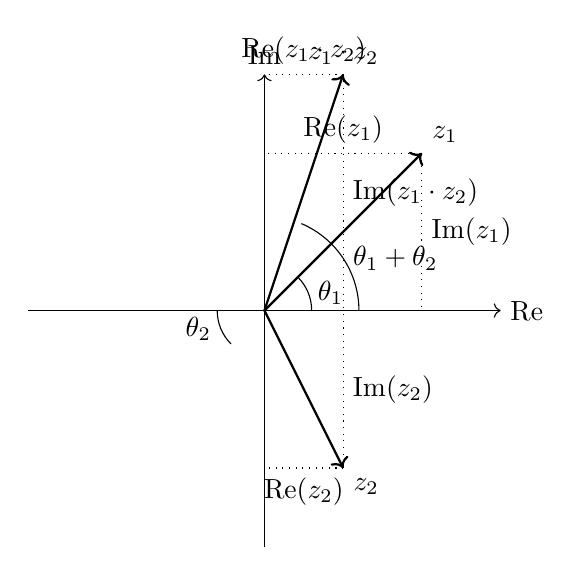
\begin{tikzpicture}[scale=2]
		% axes
		\draw[->] (-1.5,0) -- (1.5,0) node[right] {$\text{Re}$};
		\draw[->] (0,-1.5) -- (0,1.5) node[above] {$\text{Im}$};
		
		% z1
		\draw[->,thick] (0,0) -- (1,1) node[above right] {$z_1$};
		\draw[dotted] (1,1) -- (1,0) node[midway,right] {$\operatorname{Im}(z_1)$};
		\draw[dotted] (1,1) -- (0,1) node[midway,above] {$\operatorname{Re}(z_1)$};
		\draw (0.3,0) arc (0:45:0.3) node[midway,right] {$\theta_1$};
		
		% z2
		\draw[->,thick] (0,0) -- (0.5,-1) node[below right] {$z_2$};
		\draw[dotted] (0.5,-1) -- (0.5,0) node[midway,right] {$\operatorname{Im}(z_2)$};
		\draw[dotted] (0.5,-1) -- (0,-1) node[midway,below] {$\operatorname{Re}(z_2)$};
		\draw (-0.3,0) arc (180:225:0.3) node[midway,left] {$\theta_2$};
		
		% z1*z2
		\draw[->,thick] (0,0) -- (0.5,1.5) node[above] {$z_1 \cdot z_2$};
		\draw[dotted] (0.5,1.5) -- (0.5,0) node[midway,right] {$\operatorname{Im}(z_1\cdot z_2)$};
		\draw[dotted] (0.5,1.5) -- (0,1.5) node[midway,above] {$\operatorname{Re}(z_1\cdot z_2)$};
		\draw (0.6,0) arc (0:67:0.6) node[midway,right] {$\theta_1+\theta_2$};
		
		% braces
		%\draw[decorate,decoration={brace,amplitude=5pt},xshift=-4pt,yshift=0pt]
		%(0.5,0) -- (0.5,1.5) node [black,midway,xshift=-8pt] {$r_1 r_2$};
		%\draw[decorate,decoration={brace,amplitude=5pt},xshift=0pt,yshift=4pt]
		%(0,1.5) -- (0.5,1.5) node [black,midway,yshift=10pt] {$r_1 r_2$};
		\end{tikzpicture}
	\end{center}
	
	
	% End document
\end{document}